\chapter{Applicazioni}
\label{ch:applicazioni}

L'utente tramite l'interfaccia ha la possibilità di scegliere tra alcuni potenziali pre-impostati:
\begin{itemize}[nolistsep]
    \item particella libera,
    \item oscillatore armonico,
    \item buca e barriera finita di potenziale,
    \item gradino di potenziale,
    \item barriera coulombiana semplificata ,
    \item potenziale \textsl{reflectionless} di P\"oschl-Teller,
    \item barriera infinita.
\end{itemize}
Da combinare con i seguenti stati iniziali:
\begin{itemize}[nolistsep]
    \item pacchetto gaussiano di onde piane, 
    \item autostati dell'oscillatore armonico e loro sovrapposizioni,
    \item stati coerenti,
    \item pacchetto gaussiano di autotati del potenziale di PL.
\end{itemize}
In questa sezione non solo si riportano alcuni dei risultati ottenuti partendo dagli stati sopracitati, ma anche altre soluzioni di particolare interesse.


\section{Buca finita di potenziale}
\label{sec:finite_hole}

La buca finita è definita tramite
\begin{equation}
    \centering
    V(x) =
    \begin{cases}
        \; -V_0  \quad &\text{per} \quad a \le x \le b \\
        \; 0 \qquad &\text{altrove}      \; \text{.}
    \end{cases}
\end{equation}
La soluzione di questo problema permette di mettere in evidenza un fenomeno caratteristico della meccanica quantistica: la riflessione di una particella può avvenire anche in corrispondenza di un caduta di potenziale. 
%ben riassunto nella frase di David Jeffrey Griffiths: \textcolor{red}{\dots \dots \dots}
Un tale comportamento è una totale novità rispetto alla meccanica classica. Secondo le equazioni di Newton $m \ddot{\vec{x}} = -\nabla U(\vec{x}, t)$, per cui risulta che in corrispondenza di una differenza di potenziale negativa la particella subisca con certezza una determinata accelerazione nella direzione del moto. In meccanica quantistica questo non è certo che accada, come mostrato in figura (\ref{fig:finite_hole}), infatti esiste una probabilità diversa zero che la particella si trovi nella zona precedente la buca con momento opposto.

\begin{figure}
    \centering
    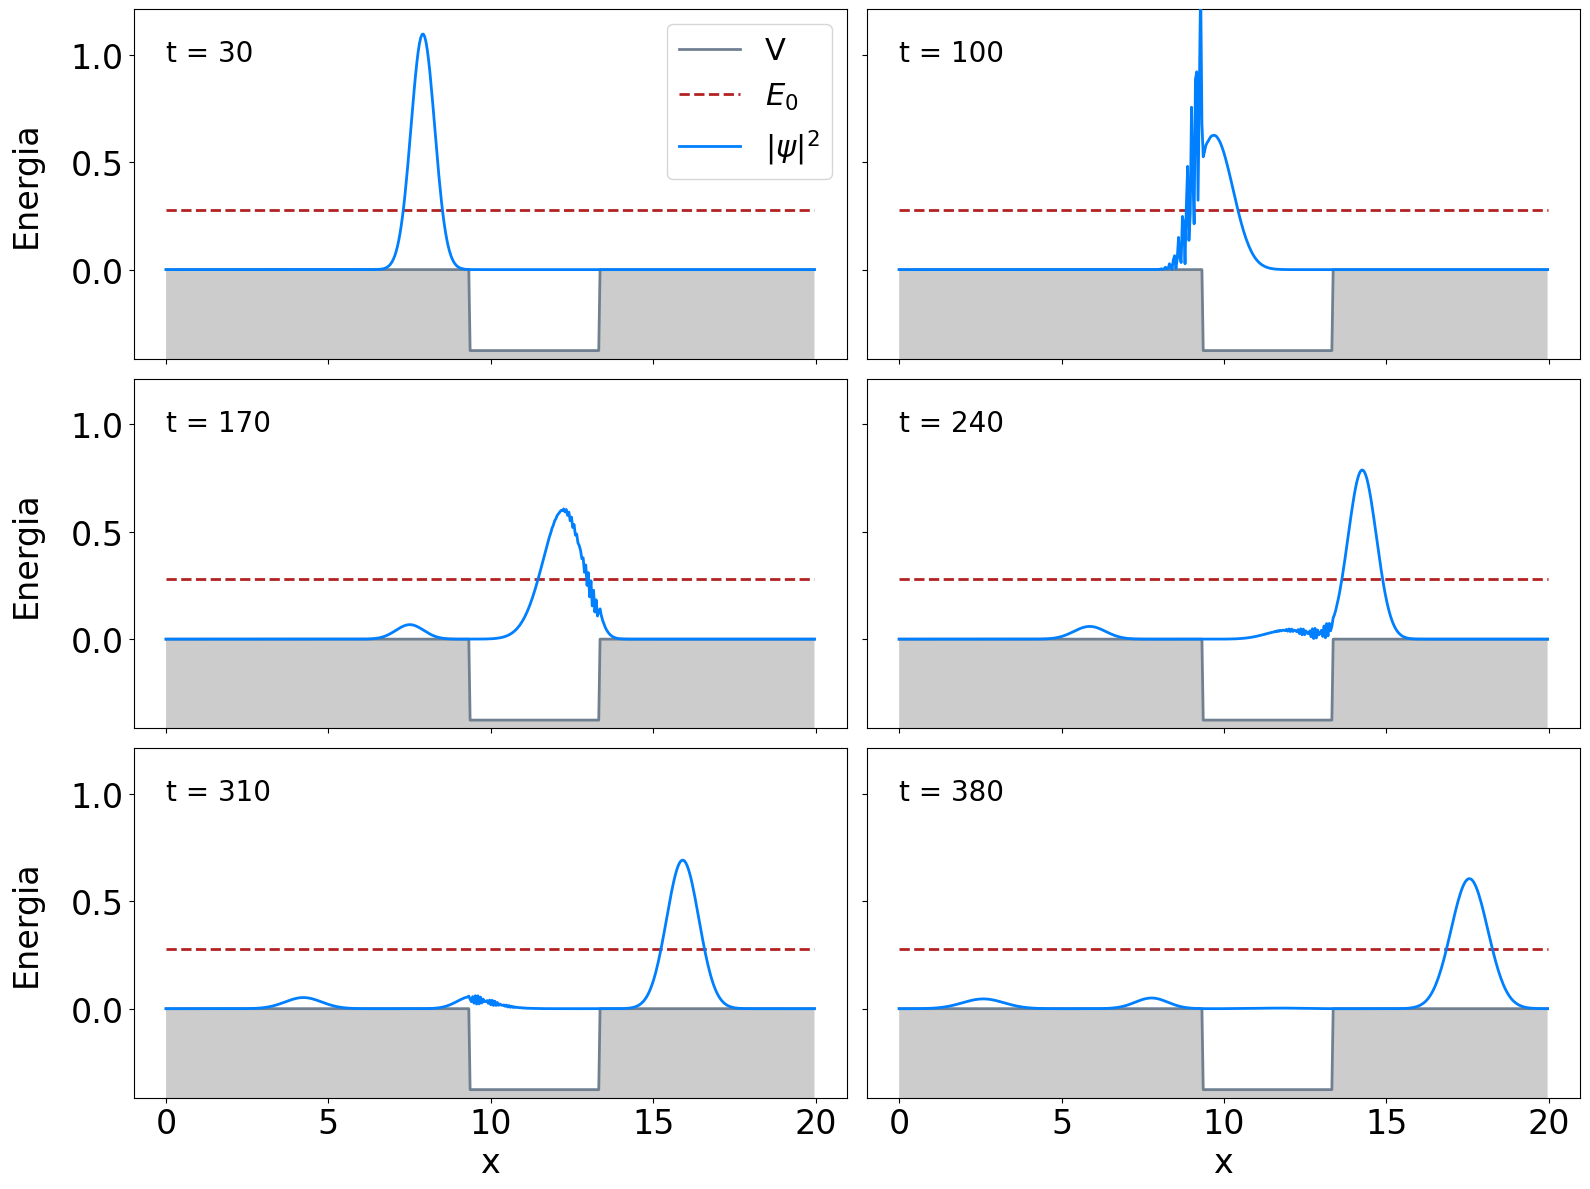
\includegraphics[width = \textwidth]{immagini/hole.png}
    \caption{Evoluzione di un pacchetto gaussiano di onde piano che interagisce con una buca finita di potenziale, si noti il fatto che parte dell'onda viene riflessa, cosa non prevista in meccanica classica.}
    \label{fig:finite_hole}
\end{figure}

\section{Barriera coulombiana semplificata}
\label{sec:coulomb}

È noto come, in prima approssimazione, il potenziale caratteristico per le particelle contenute nel nucleo abbia una forma del tipo
\begin{equation}
    \centering
    V(r) = 
    \begin{cases}
        \, - V_{N} \quad &\text{per} \quad r \le \tilde{R} \\
        \, (Z \, e_0^2) \ (4 \pi \, \epsilon_0) \;\; r^{-1} \quad &\text{per} \quad r > \tilde{R}      \; \text{.}
    \end{cases}
    \label{eq:C_pot}
\end{equation} 
Nel codice è stato implementato un potenziale con lo stesso andamento 
\begin{equation}
    \centering
    V(x) = 
    \begin{cases}
        \, 0 \quad &\text{per} \quad x \le \tilde{x} \\
        \, \left( x - \tilde{x} - (1 / V_0)\right)^{-1} \quad &\text{per} \quad x > \tilde{x}  \; \text{,}
    \end{cases}
    \label{eq:tunnel}
\end{equation} 
per mettere in evidenza un altro fenomeno caratteristico della meccanica quantistica: l'effetto tunnel.
Fenomeno attraverso il quale si giustifica l'espulsione di particelle dal nucleo durante i decadimenti-$\alpha$.
In figura (\ref{fig:tunnel}) si può vedere che nonostante la particella non abbia l'energia sufficiente ad oltrepassare la barriera, \textcolor{red}{secondo la meccanica classica}, una parte della funzione d'onda viene trasmessa.

\begin{figure}
    \centering
    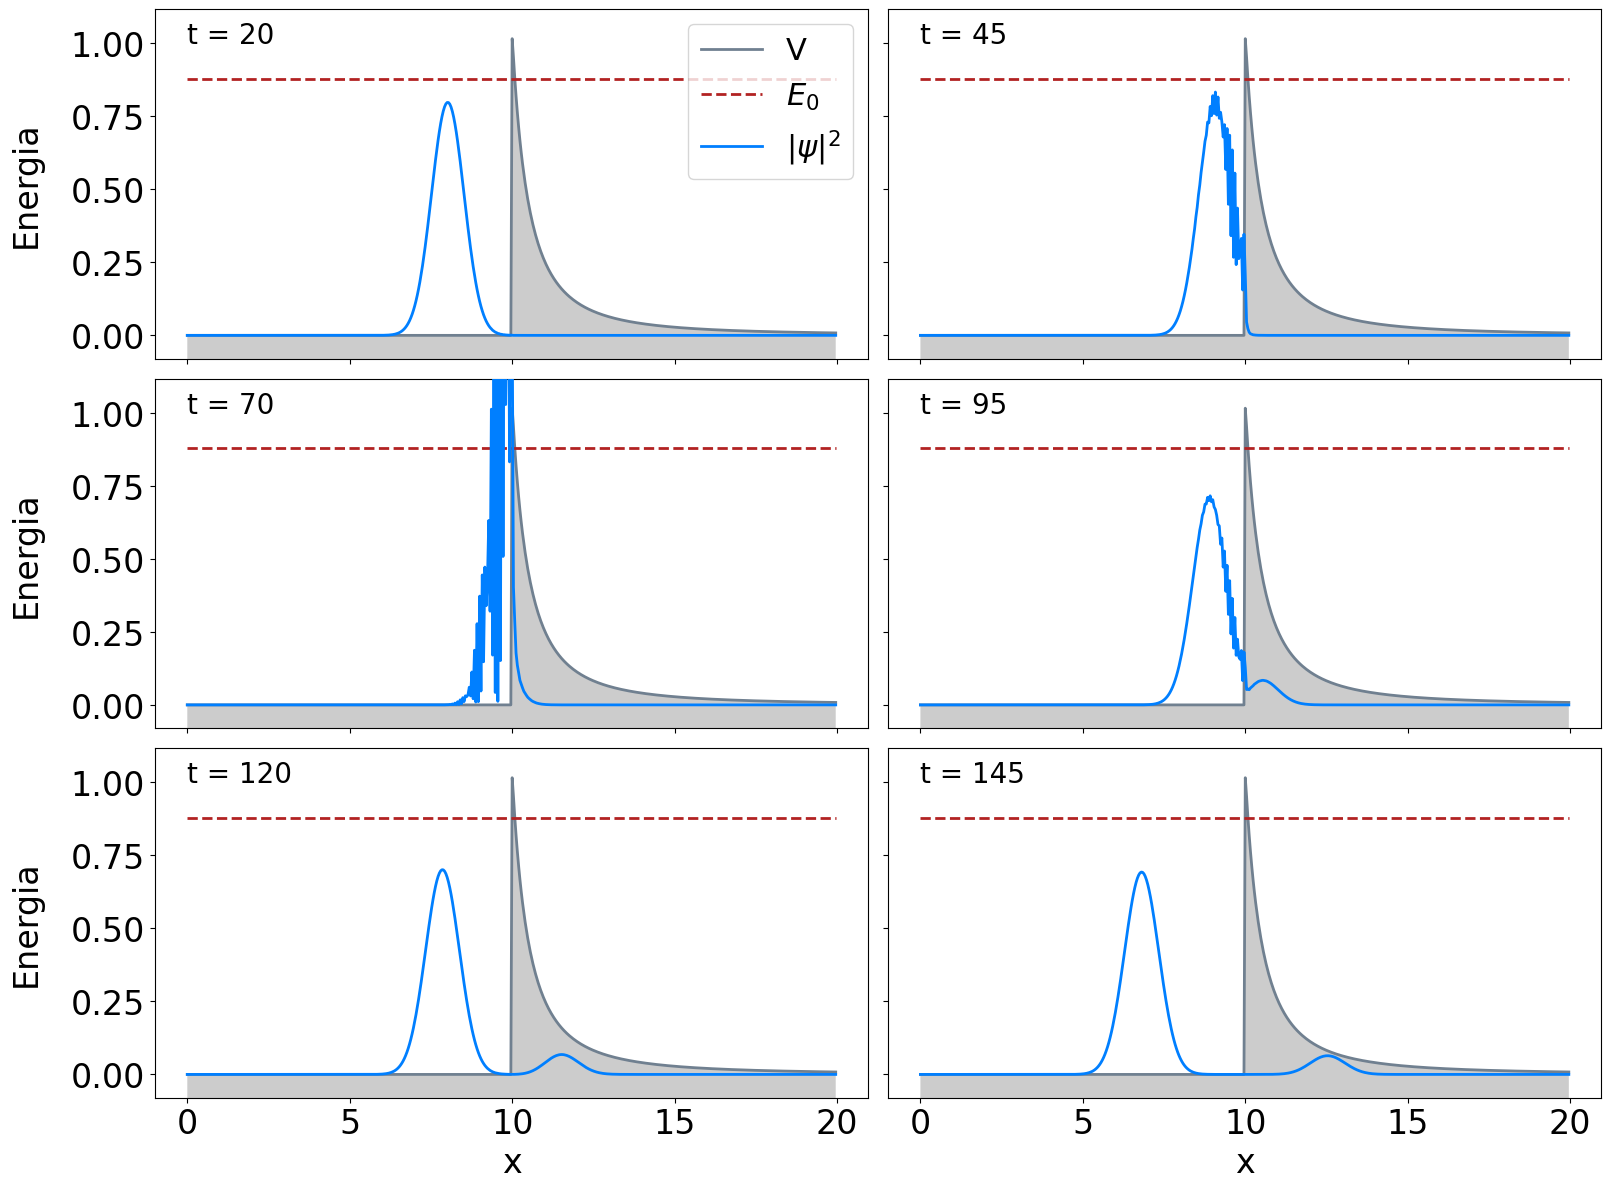
\includegraphics[width = \textwidth]{immagini/tunnel.png}
    \caption{Visualizzazione grafica dell'effetto tunnel per un potenziale Coulombiano.}
    \label{fig:tunnel}
\end{figure}


\section{Pacchetto gaussiano di onde piane in oscillatore armonico}
\label{sec:Wp_arm}

Si ricorda che il comportamento classico di un particella soggetta ad un potenziale armonico è del tutto simile al comportamento di uno stato coerente, come già valutato in sezione (\ref{sec:coherent}).
In questa sezione si vogliono evidenziare le differenze tra uno stato coerente e l'evoluzione di un pacchetto gaussiano di onde piane a cui è associata la stessa energia.
Come si può vedere in figura (\ref{fig:co_vs_WP}), la dinamica del centro di massa del pacchetto di onde piane è facilmente interpretabile tramite la meccanica classica. Infatti il valor medio $\expval{x}$ del pacchetto si sovrappone al valore medio dello stato coerente. D'altra parte mentre gli stati coerenti mantegono le dimensioni del profilo gaussiano, il pacchetto di onde piane subisce continue defomazioni lungo il moto. Emerge un comportamento puramente quantistico per cui la varianza del pacchetto subisce delle contrazioni e delle dilatazioni periodiche di periodo pari alla metà di quello dell'oscillatore armonico classico. \cite{Tsuru:gaus_harmonic}   

\begin{figure}
    \centering
    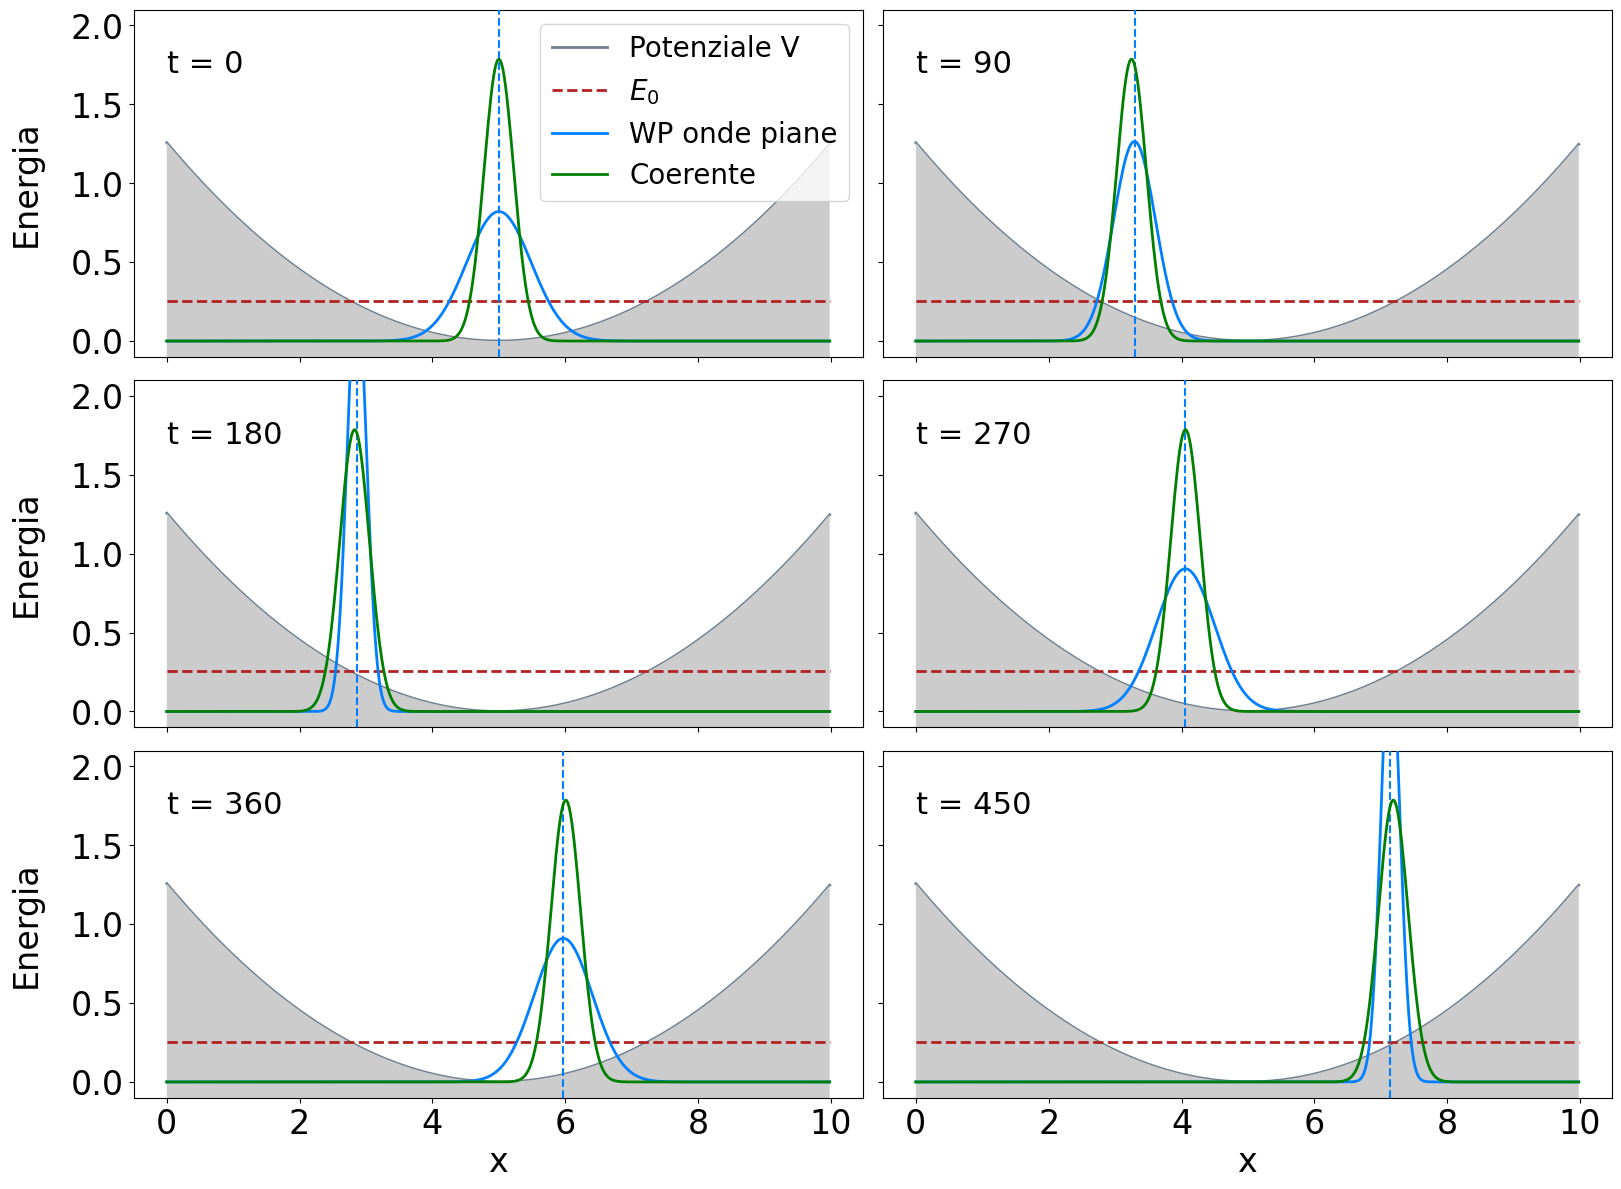
\includegraphics[width = \textwidth]{immagini/coherent_vs_WP.png}
    \caption{Confronto tra l'evoluzione di uno stato coerente e un pacchetto gaussiano di onde piane.}
    \label{fig:co_vs_WP}
\end{figure}

\section{Pacchetto gaussiano di onde piane in potenziale di P\"oschl-Teller}
\label{sec:Wp_PL}

Se si considera un pacchetto gaussiano di onde piane che attraversa un potenziale di P\"oschl-Teller, risulterà che questo verrà interamente trasmesso, come sottolineato in sezione (\ref{sec:RL}).
Si può studiare la deformazione subita dal pacchetto durante il moto e confrontarla con un pacchetto di autostati di PL e l'evoluzione libera.
Come si può riscontrare in figura (\ref{fig:PL_conf}), il pacchetto viene deformato in maniera simile al pacchetto di autosati, subisce un'accelerazione e si ottiene un pacchetto contratto rispetto all'evoluzione libera. Le linee verticali in figura (\ref{fig:PL_conf}) rappresentano il valore medio $\expval{x}$ della corrispettiva funzione d'onda: risulta che il pacchetto d'onde di autostati possiede una velocità di gruppo più alta rispetto al pacchetto gaussiano e risente maggiormente degli effetti del potenziale, è infatti accelerato più velocemente.\cite{Mousavi:PL_WP}

Si è inoltre confrontata l'evoluzione libera di un pacchetto gaussiano di onde piane con la sua evoluzione nel potenziale PL. Risulta che il pacchetto d'onde subisca una deformazione che lo trasla più velocemente rispetto alla propagazione libera lasciandolo più contratto.\cite{Lecker:RL}
\textcolor{red}{ Se si immagina di implementare un reticolo ben dimensionato si potrebbe costruire una macchina che trasporta le particelle da un lato all'altro in maniera molto più efficiente, vedi figura \dots.} 

\begin{figure}
    \centering
    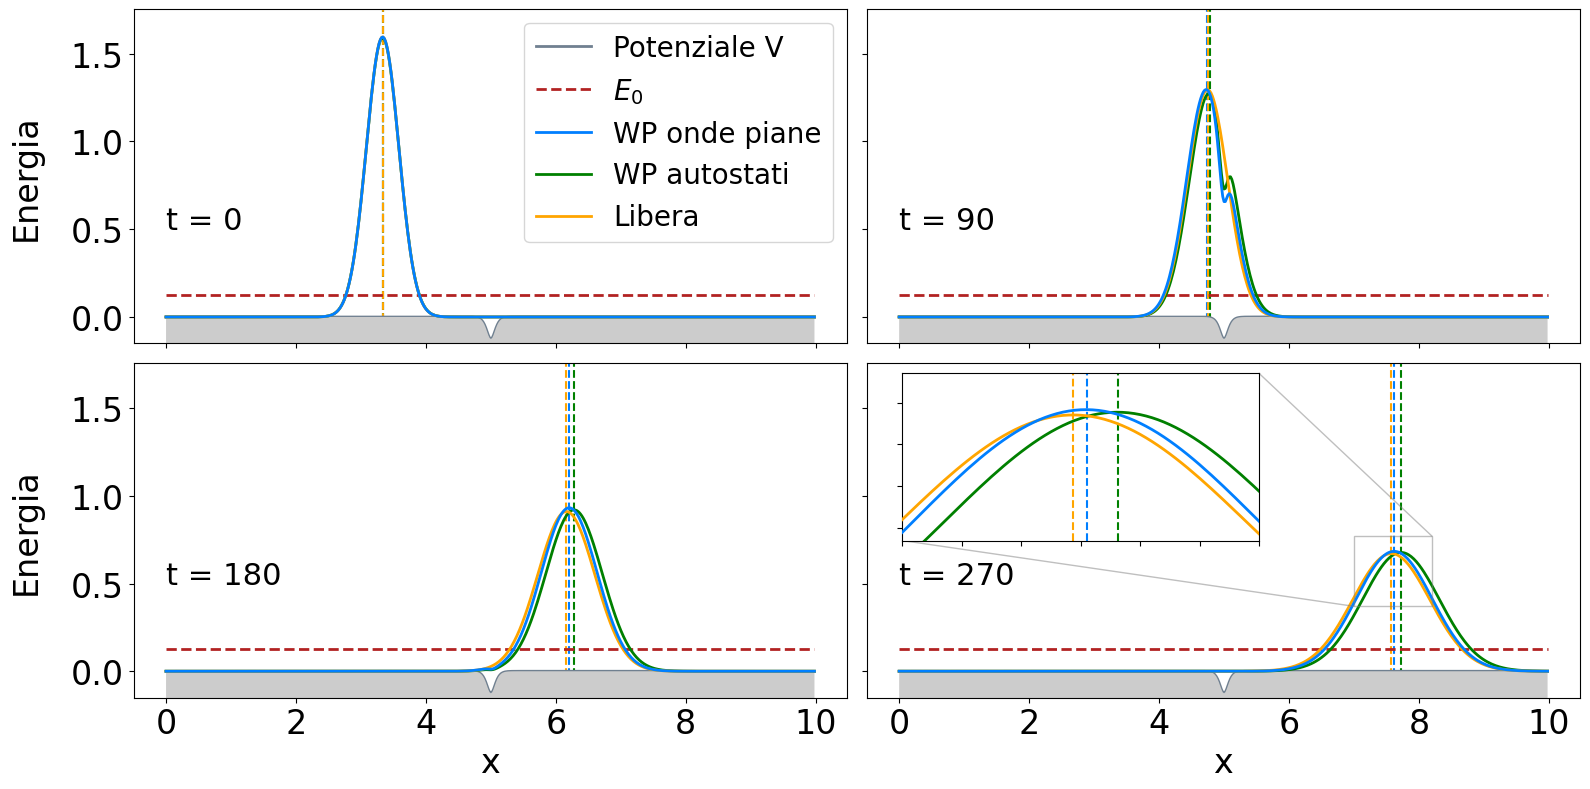
\includegraphics[width = \textwidth]{immagini/PL_num.png}
    \caption{Confronto tra l'evoluzione di uno stato coerente e un pacchetto gaussiano di onde piane.}
    \label{fig:PL_conf}
\end{figure}

\begin{figure}
    \centering
    \includegraphics[width = \textwidth]{immagini/PL_num_zoom.png}
    \caption{Confronto tra l'evoluzione di uno stato coerente e un pacchetto gaussiano di onde piane.}
    \label{fig:PL_conf_zoom}
\end{figure}

\section{Barriera infinita}
\label{sec:inf}

Come riportato in sezione \ref{sec:limits}, non è possibile definire potenziali che non rispettino l'eq. (\ref{eq:V_max}). Il caso particolare della barriera infinita 
\begin{equation}
    V(x) = 
    \begin{cases}
        0 \quad &\text{per} \quad x < x_v \\
        \infty \quad &\text{per} \quad x \geq x_v \; \text{,}
    \end{cases}
    \label{eq:pot_inf}
\end{equation}
è però risolvibile lasciando evolvere un pacchetto opportunamente costruito in un potenziale costante $V = 0$. La presenza di una barriera infinita si traduce matematicamente nell'affermare che 
\begin{equation}
    \psi(x_v, t) = 0 \quad \forall t \; \text{,}
    \label{eq:cond_dir}
\end{equation}
nota anche come condizione al bordo di Dirichlet. 
Se si considera la funzione d'onda antisimmetrica rispetto a $x_v$ di $\psi(x,t)$, costruita con
\begin{equation}
    \psi_{\text{ANT}}(x -x_v, t) =  - \psi(x_v - x , t) \; \text{,} 
\end{equation}    
questa, in un potenziale libero, evolverà in direzione opposta rispetto a $\psi$. Nel momento in cui si considera la sovrapposizione dei due, $\Psi(x,t) = \psi(x, t) + \psi_{\text{ANT}}(x, t)$, si ottiene per costruzione che l'eq. (\ref{eq:cond_dir}) è identicamente verificata $\forall t$. 
La soluzione del problema proposto risulta essere $\Psi(x,t)$ valutata nel'intervallo $(-\infty, 0]$. In figura (\ref{fig:inf}) si riportano i risultati di una simulazione numerica per un pacchetto gaussiano in un potenziale di eq. (\ref{eq:pot_inf}), risolto con il metodo appena descritto.

\begin{figure}
    \centering
    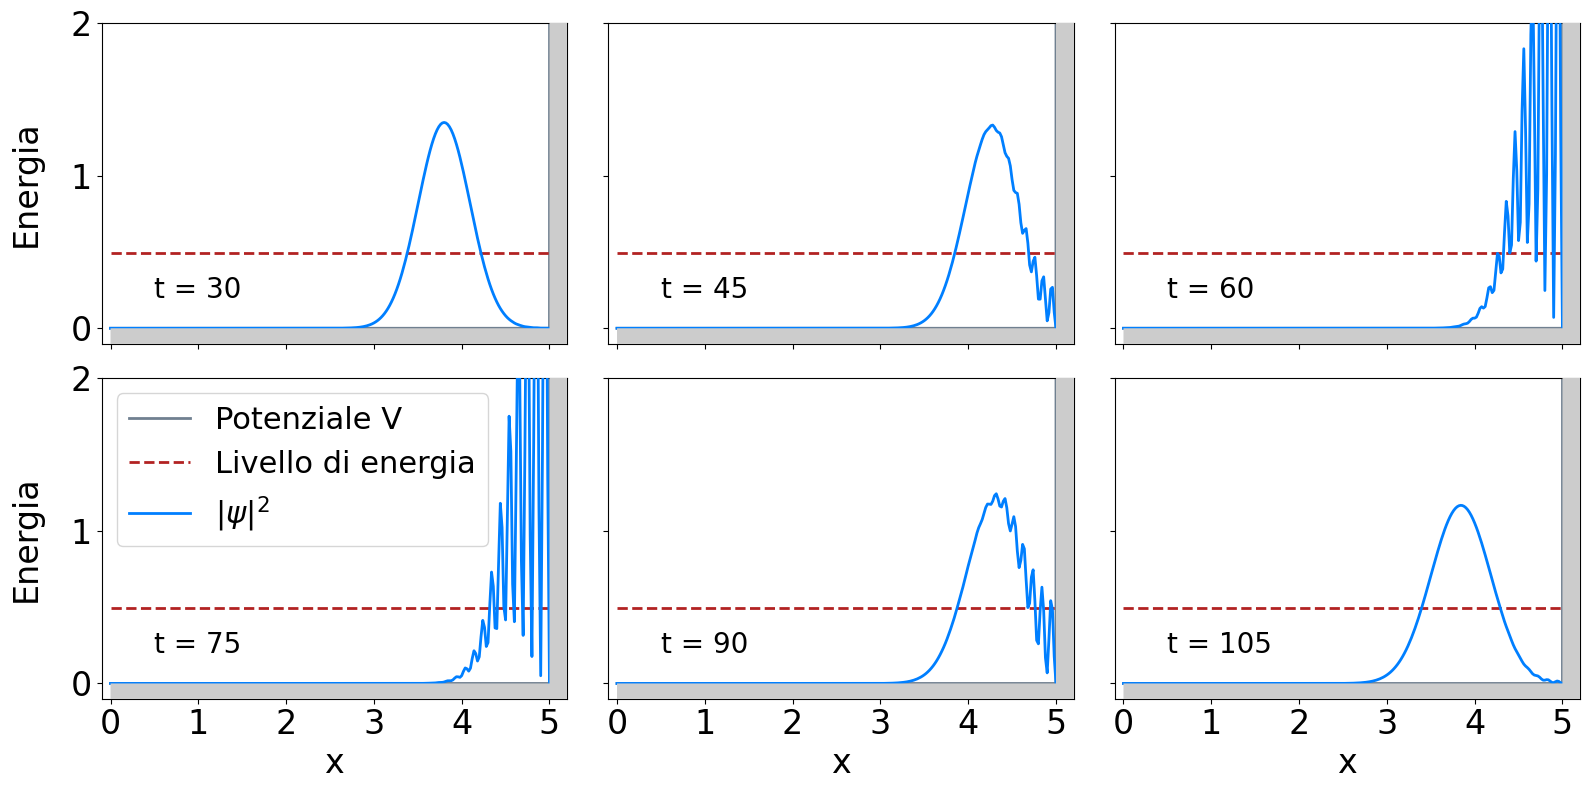
\includegraphics[width = \textwidth]{immagini/inf.png}
    \caption{Evoluzione di un pacchetto gaussiano di onde piano che interagisce con una barriera di potenziale infinita. \textcolor{red}{Se può essere interessante posso sovrappore questa soluzione con la soluzione di un potenziale step con $V_0 \approx V_{MAX}$}}
    \label{fig:inf}
\end{figure}

\section{Potenziale dipendente dal tempo}
\label{sec:t_dep}

Come anticipato è possibile risolvere anche problemi con potenziale dipendente dal tempo.
Come esempio si è scelto di implemenatare un potenziale 
\begin{equation}
   \centering
   V(x) = \alpha \, (x-x_0)^2 +  \frac{| \sin (\omega_v  \, t) |} {1 + \beta \, (x-x_0)^2} \, \text{.}
\end{equation}
Come si può vedere in figura (\ref{fig:t-dep}) è evidente come la funzione d'onda reagisca al potenziale mentre questo cambia forma.

\begin{figure}
   \centering
    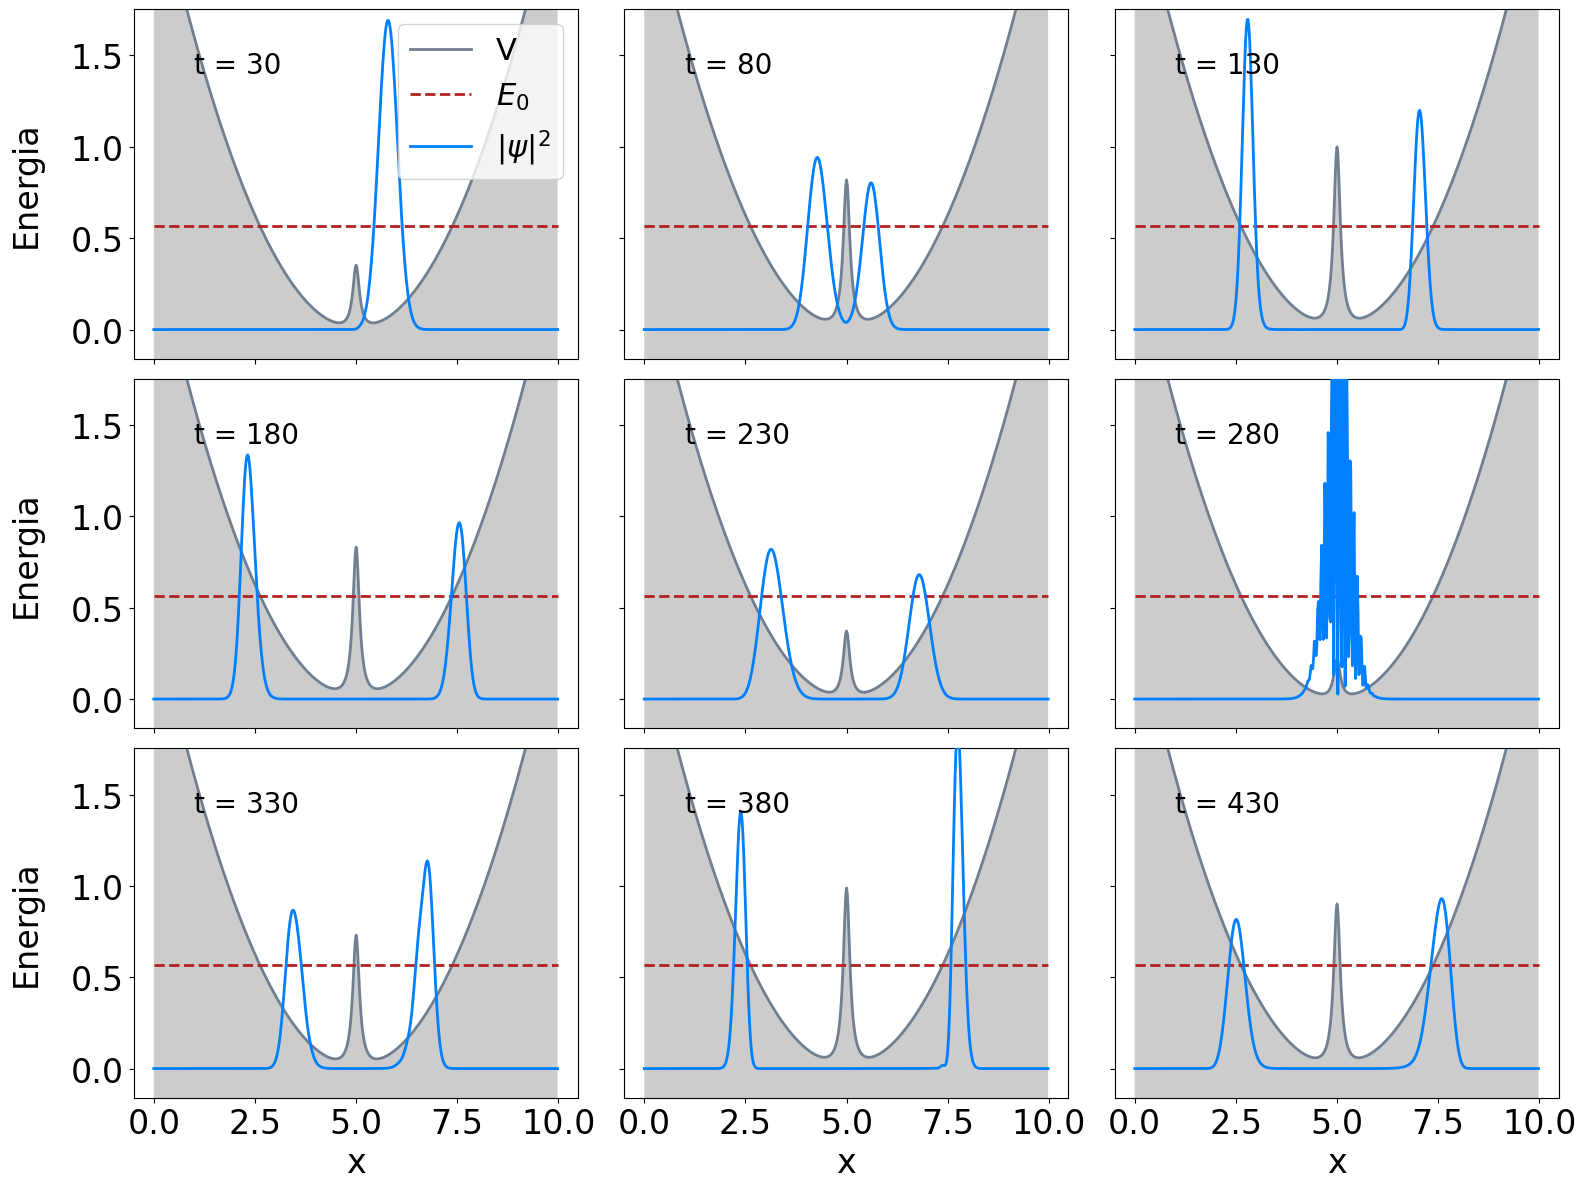
\includegraphics[width = \textwidth]{immagini/t-dep.png}
    \caption{Evoluzione di un pacchetto gaussiano di onde piano che interagisce con un potenziale dipendente dal tempo. Notare come per $t \, \approx \, 80$ la funzione d'onda venga separata tra le due regioni per poi sovrapporsi nuovamente per  $t \, \approx \, 280$ }
    \label{fig:t-dep}
\end{figure}

   
   




